\documentclass[tikz,border=10pt]{standalone}

\usepackage{tikz}
\usetikzlibrary{arrows.meta,positioning}

\tikzset{
    box/.style={
        draw, rounded corners, thick,
        minimum width=3.8cm, minimum height=1cm,
        align=center
    }
}

\begin{document}

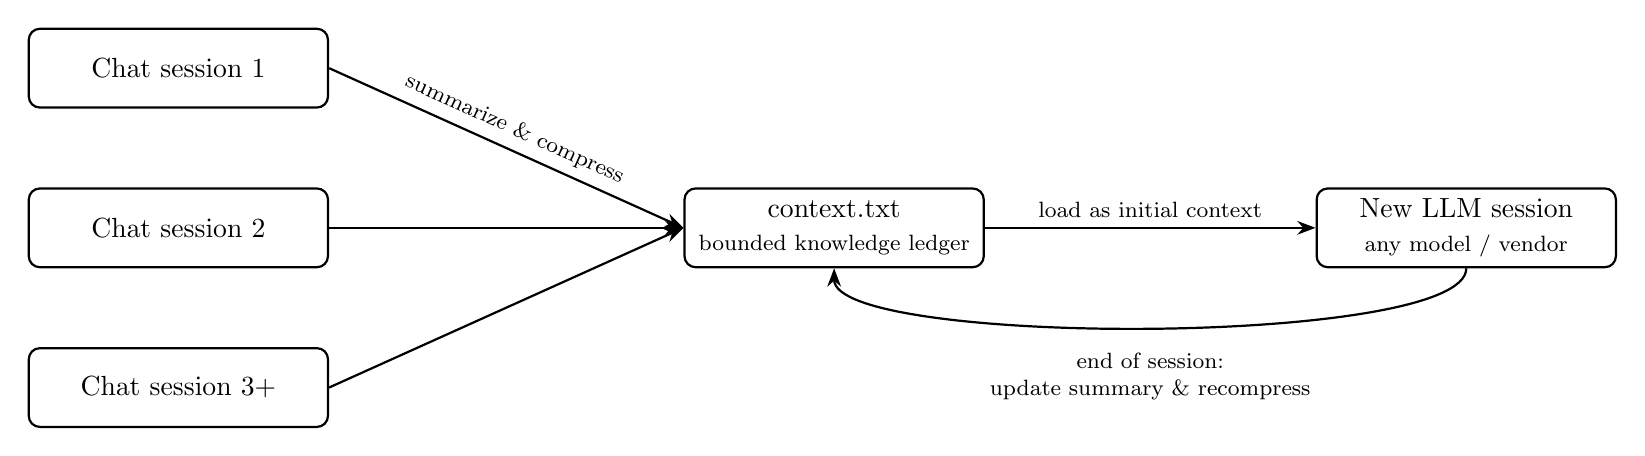
\begin{tikzpicture}[>=Stealth, node distance=1.8cm]

% Boxes
\node[box] (c1) {Chat session 1};
\node[box, below=1.0cm of c1] (c2) {Chat session 2};
\node[box, below=1.0cm of c2] (c3) {Chat session 3+};

\node[box, right=4.5cm of c2] (ctx) {context.txt\\{\footnotesize bounded knowledge ledger}};
\node[box, right=4.2cm of ctx] (next) {New LLM session\\{\footnotesize any model / vendor}};

% Arrows from sessions to ledger
\draw[->, thick] (c1.east) -- node[above, sloped]{\footnotesize summarize \& compress} (ctx.west);
\draw[->, thick] (c2.east) -- (ctx.west);
\draw[->, thick] (c3.east) -- (ctx.west);

% Arrow ledger -> next session
\draw[->, thick] (ctx.east) -- node[above]{\footnotesize load as initial context} (next.west);

% Arrow back for update loop
\draw[->, thick]
    (next.south) .. controls +(0,-1.0) and +(0,-1.0) ..
    node[midway, below=0.2cm, align=center, font=\footnotesize]
        {end of session:\\ update summary \& recompress}
    (ctx.south);

\end{tikzpicture}

\end{document}

